\begin{minipage}{0.75\linewidth}
\begin{figure}[h]
    \centering
    \begin{adjustbox}{max width=1.0\linewidth, keepaspectratio}
        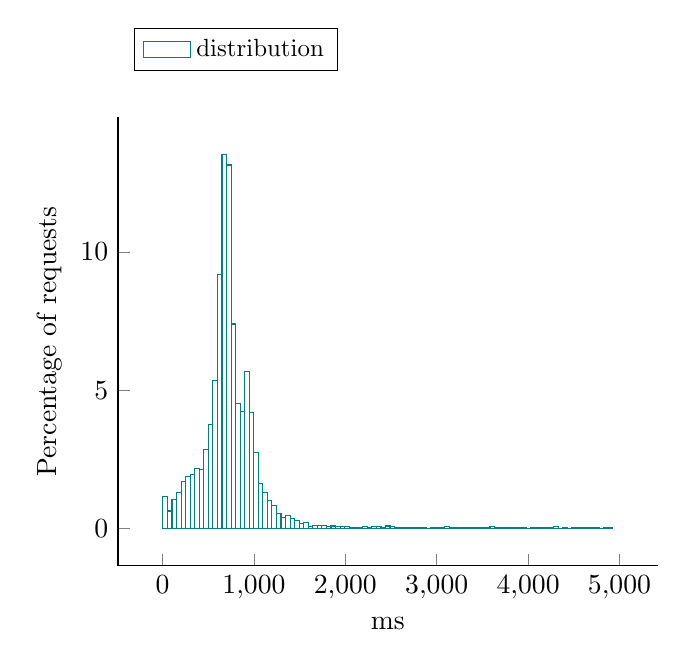
\begin{tikzpicture}
            \begin{axis}[ylabel = Percentage of requests, 
xlabel = ms, 
legend style = {nodes={scale=0.9, transform shape}, at={(0.03,1.2)}, anchor=north west, draw=black, fill=white, align=left, legend columns=3},
area style, mark size = 0pt,
 cycle list name = exotic,
  axis lines* = left]
		\addplot +[ybar interval] coordinates {
			 (4, 1.15481)
			 (53.71, 0.62422)
			 (103.42, 1.02996)
			 (153.13, 1.30046)
			 (202.84, 1.6958)
			 (252.55, 1.88306)
			 (302.26, 1.95589)
			 (351.97, 2.17437)
			 (401.68, 2.13275)
			 (451.39, 2.86101)
			 (501.1, 3.75572)
			 (550.81, 5.34748)
			 (600.52, 9.17603)
			 (650.23, 13.5248)
			 (699.94, 13.1502)
			 (749.65, 7.397)
			 (799.36, 4.51519)
			 (849.07, 4.21348)
			 (898.78, 5.6804)
			 (948.49, 4.18227)
			 (998.2, 2.75697)
			 (1047.91, 1.61257)
			 (1097.62, 1.31086)
			 (1147.33, 1.00916)
			 (1197.04, 0.821889)
			 (1246.75, 0.551394)
			 (1296.46, 0.395339)
			 (1346.17, 0.468165)
			 (1395.88, 0.353725)
			 (1445.59, 0.270495)
			 (1495.3, 0.176862)
			 (1545.01, 0.19767)
			 (1594.72, 0.0520183)
			 (1644.43, 0.11444)
			 (1694.14, 0.11444)
			 (1743.85, 0.104037)
			 (1793.56, 0.0520183)
			 (1843.27, 0.0832293)
			 (1892.98, 0.0520183)
			 (1942.69, 0.0728256)
			 (1992.4, 0.062422)
			 (2042.11, 0.0416146)
			 (2091.82, 0.0208073)
			 (2141.53, 0.0416146)
			 (2191.24, 0.062422)
			 (2240.95, 0.0208073)
			 (2290.66, 0.0520183)
			 (2340.37, 0.062422)
			 (2390.08, 0.031211)
			 (2439.79, 0.0832293)
			 (2489.5, 0.0520183)
			 (2539.21, 0.0208073)
			 (2588.92, 0.0416146)
			 (2638.63, 0.0208073)
			 (2688.34, 0.031211)
			 (2738.05, 0.031211)
			 (2787.76, 0.0416146)
			 (2837.47, 0.0416146)
			 (2887.18, 0)
			 (2936.89, 0.031211)
			 (2986.6, 0.031211)
			 (3036.31, 0.0208073)
			 (3086.02, 0.0520183)
			 (3135.73, 0.031211)
			 (3185.44, 0.0104037)
			 (3235.15, 0.031211)
			 (3284.86, 0.0416146)
			 (3334.57, 0.0208073)
			 (3384.28, 0.0104037)
			 (3433.99, 0.0104037)
			 (3483.7, 0.0104037)
			 (3533.41, 0.0104037)
			 (3583.12, 0.0520183)
			 (3632.83, 0.0208073)
			 (3682.54, 0.0416146)
			 (3732.25, 0.0416146)
			 (3781.96, 0.0104037)
			 (3831.67, 0.031211)
			 (3881.38, 0.0416146)
			 (3931.09, 0.031211)
			 (3980.8, 0)
			 (4030.51, 0.0416146)
			 (4080.22, 0.0104037)
			 (4129.93, 0.0104037)
			 (4179.64, 0.0104037)
			 (4229.35, 0.0104037)
			 (4279.06, 0.062422)
			 (4328.77, 0)
			 (4378.48, 0.0104037)
			 (4428.19, 0)
			 (4477.9, 0.031211)
			 (4527.61, 0.0104037)
			 (4577.32, 0.0208073)
			 (4627.03, 0.0416146)
			 (4676.74, 0.0208073)
			 (4726.45, 0.0208073)
			 (4776.16, 0)
			 (4825.87, 0.0104037)
			 (4875.58, 0.0104037)
			 (4925.29, 0)
		};
\addlegendentry{distribution};
           \end{axis}
      \end{tikzpicture}
  \end{adjustbox}
  \caption{Response time distribution - req = ReadUser-3}
\end{figure}
\end{minipage}\hfill\begin{minipage}{0.18\linewidth}
\begin{table}[h]
\begin{tabular}{|cc|}
\hline
\textbf{} & \textbf{ms}\\ \hline
 \Xhline{0.005\arrayrulewidth}
min & 4\\
 \Xhline{0.005\arrayrulewidth}
max & 4975\\
 \Xhline{0.005\arrayrulewidth}
mean & 749\\
 \Xhline{0.005\arrayrulewidth}
std & 429\\
\hline
\hline
 \Xhline{0.005\arrayrulewidth}
25th & 595\\
 \Xhline{0.005\arrayrulewidth}
50th & 704\\
 \Xhline{0.005\arrayrulewidth}
75th & 867\\
 \Xhline{0.005\arrayrulewidth}
80th & 917\\
 \Xhline{0.005\arrayrulewidth}
85th & 963\\
 \Xhline{0.005\arrayrulewidth}
90th & 1037\\
 \Xhline{0.005\arrayrulewidth}
95th & 1227\\
 \Xhline{0.005\arrayrulewidth}
99th & 2799\\
\hline
\end{tabular}
\caption{Response time}
\end{table}
\end{minipage}\hfill